\section{User Roles}\label{sec:fa_roles}

\begin{figure}[H]
  \centering
  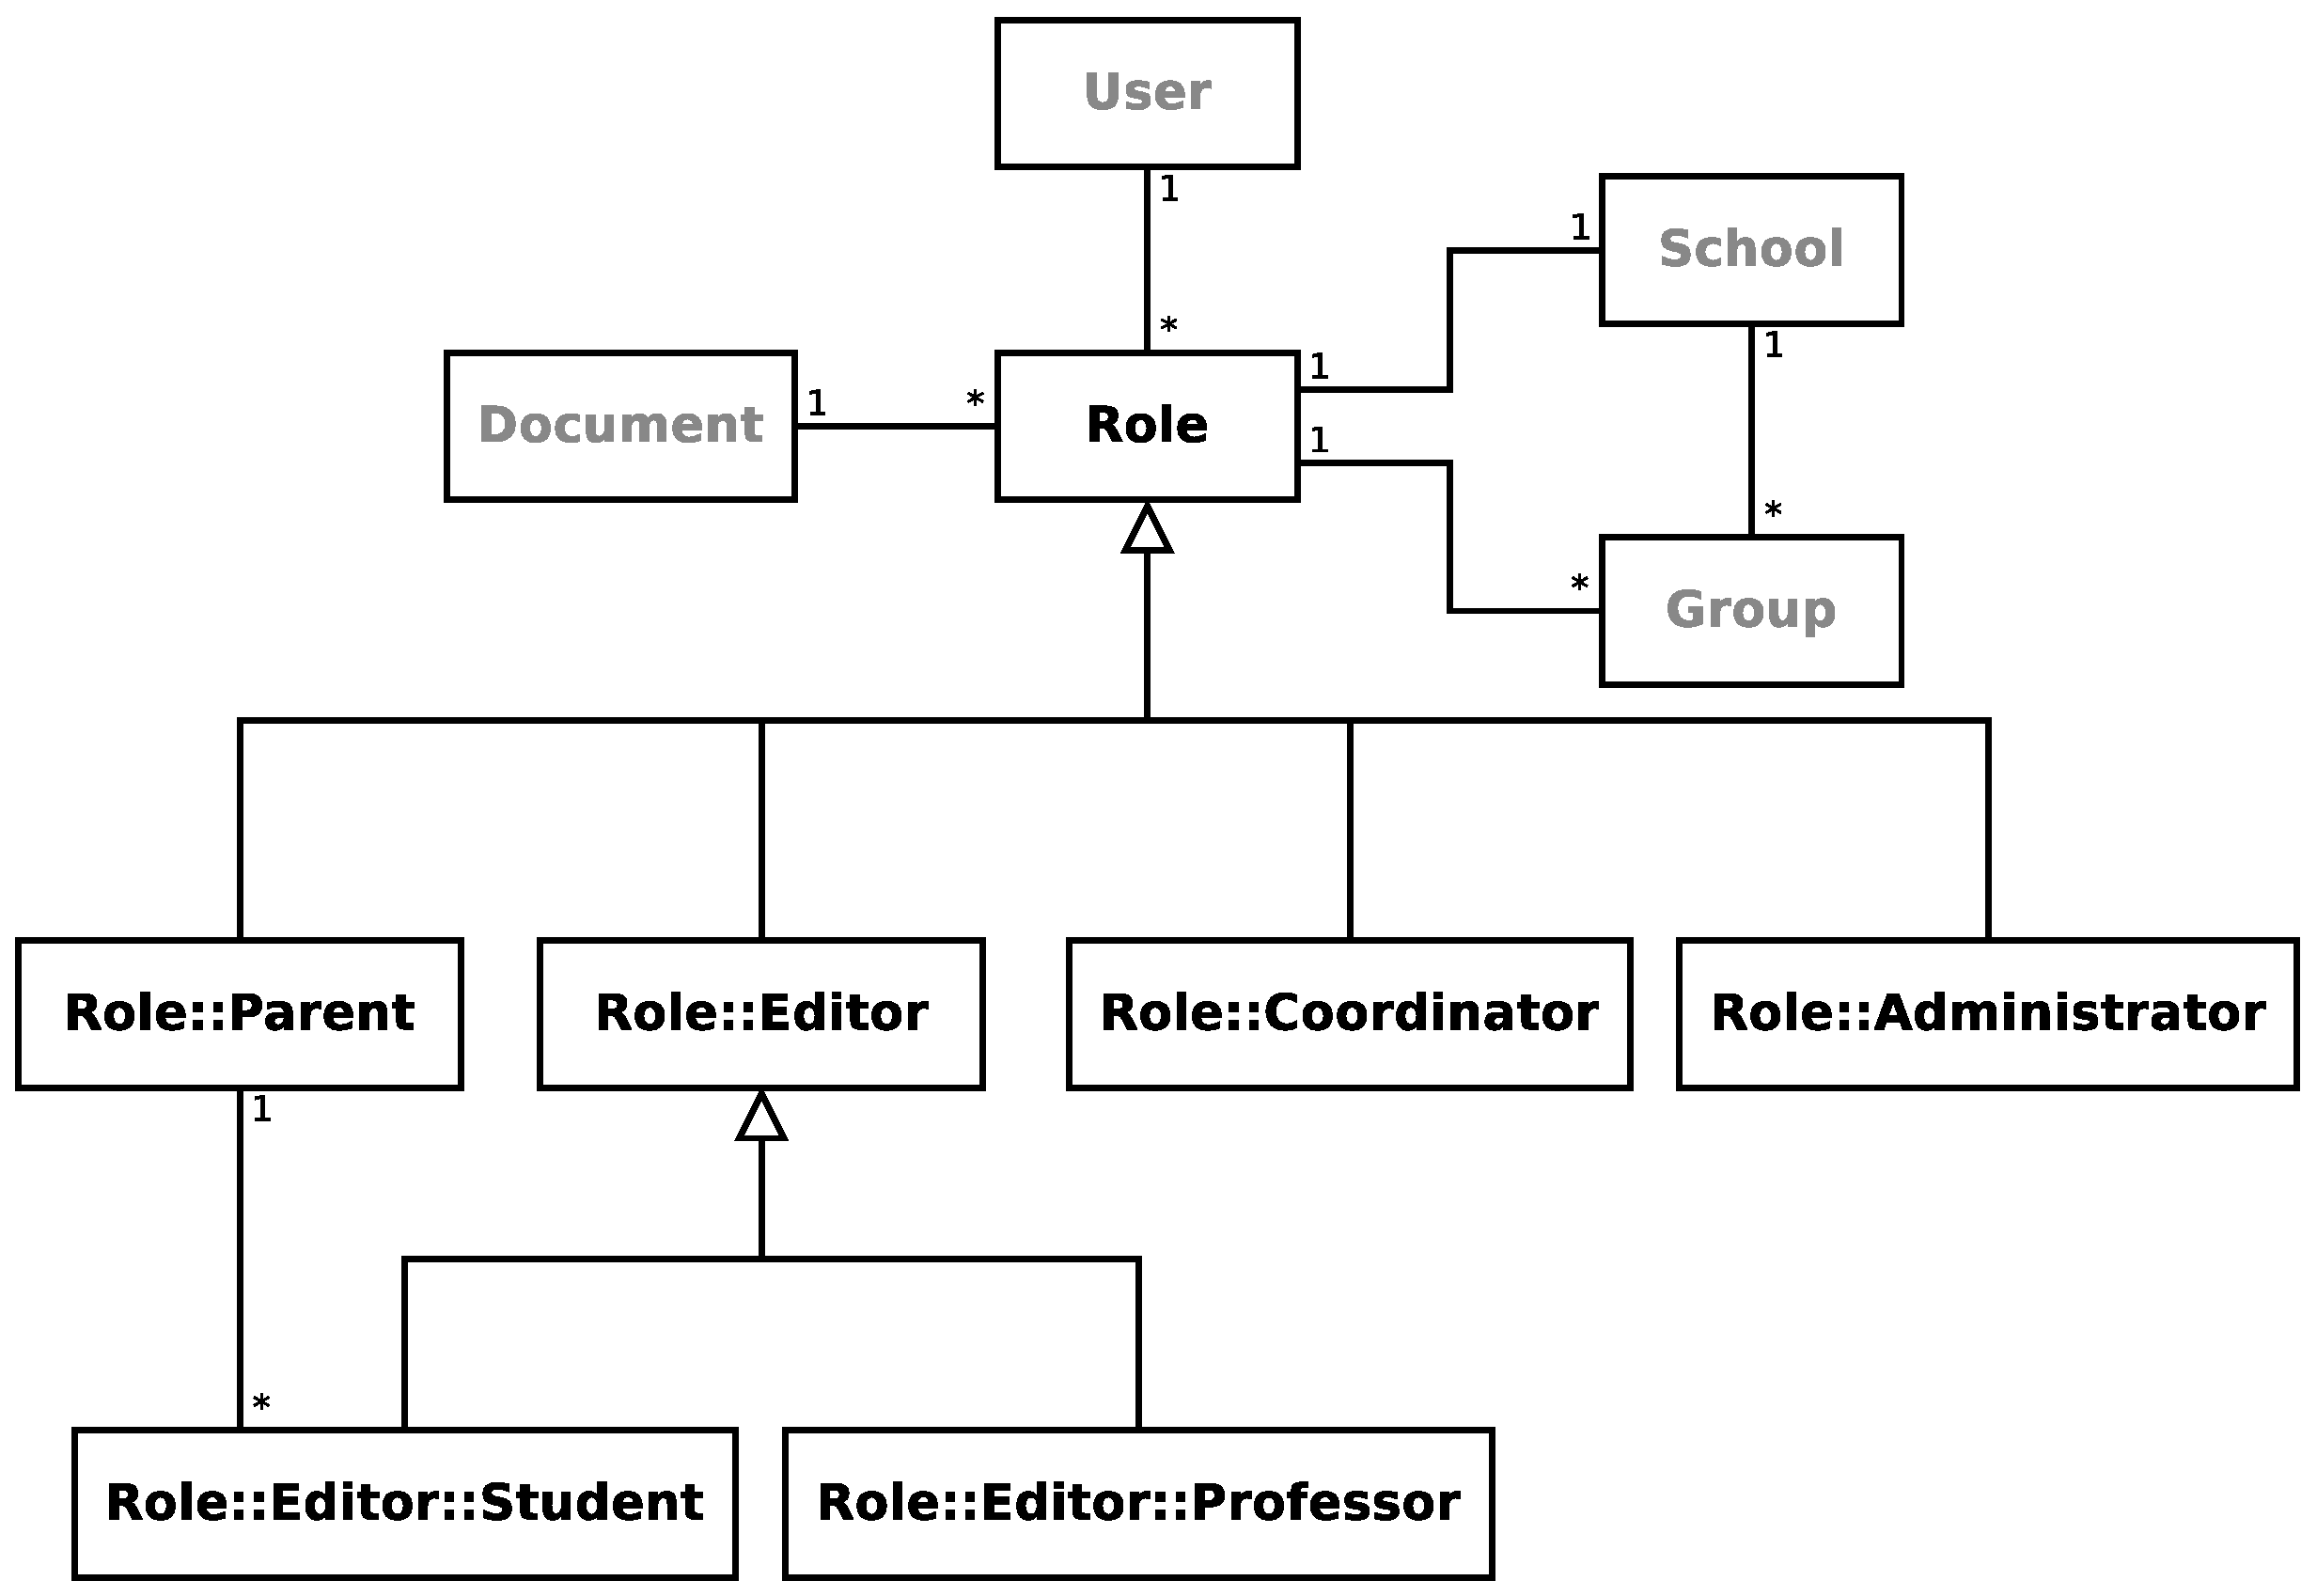
\includegraphics[width=130mm]{user_roles_current}
  \caption{Current User Roles Model}
  \label{fig:user_roles_current}
\end{figure}

\subsection{Variability Requirements}\label{sec:fa_roles_variability_requirements}

\subsection{Candidate Patterns}\label{sec:fa_roles_candidate_patterns}

\subsection{Chosen Patterns \& Rationale}\label{sec:fa_roles_chosen_patterns_rationale}

A flat Role hierarchy would allow for a more flexible authorization scheme, where a User could have one or more roles associated, depending on what actions he would be allowed to do, as shown on Fig.~\ref{fig:user_roles_conceptual}. This also makes the task of creating new roles with different authorization schemes much easier, as there is not a need to conform to any special hierarchy scheme: a new role simply means a new type of user. This clearly constrasts with the previous role's logic, where a multi-level hierarchy was in place.

\begin{figure}[H]
  \centering
  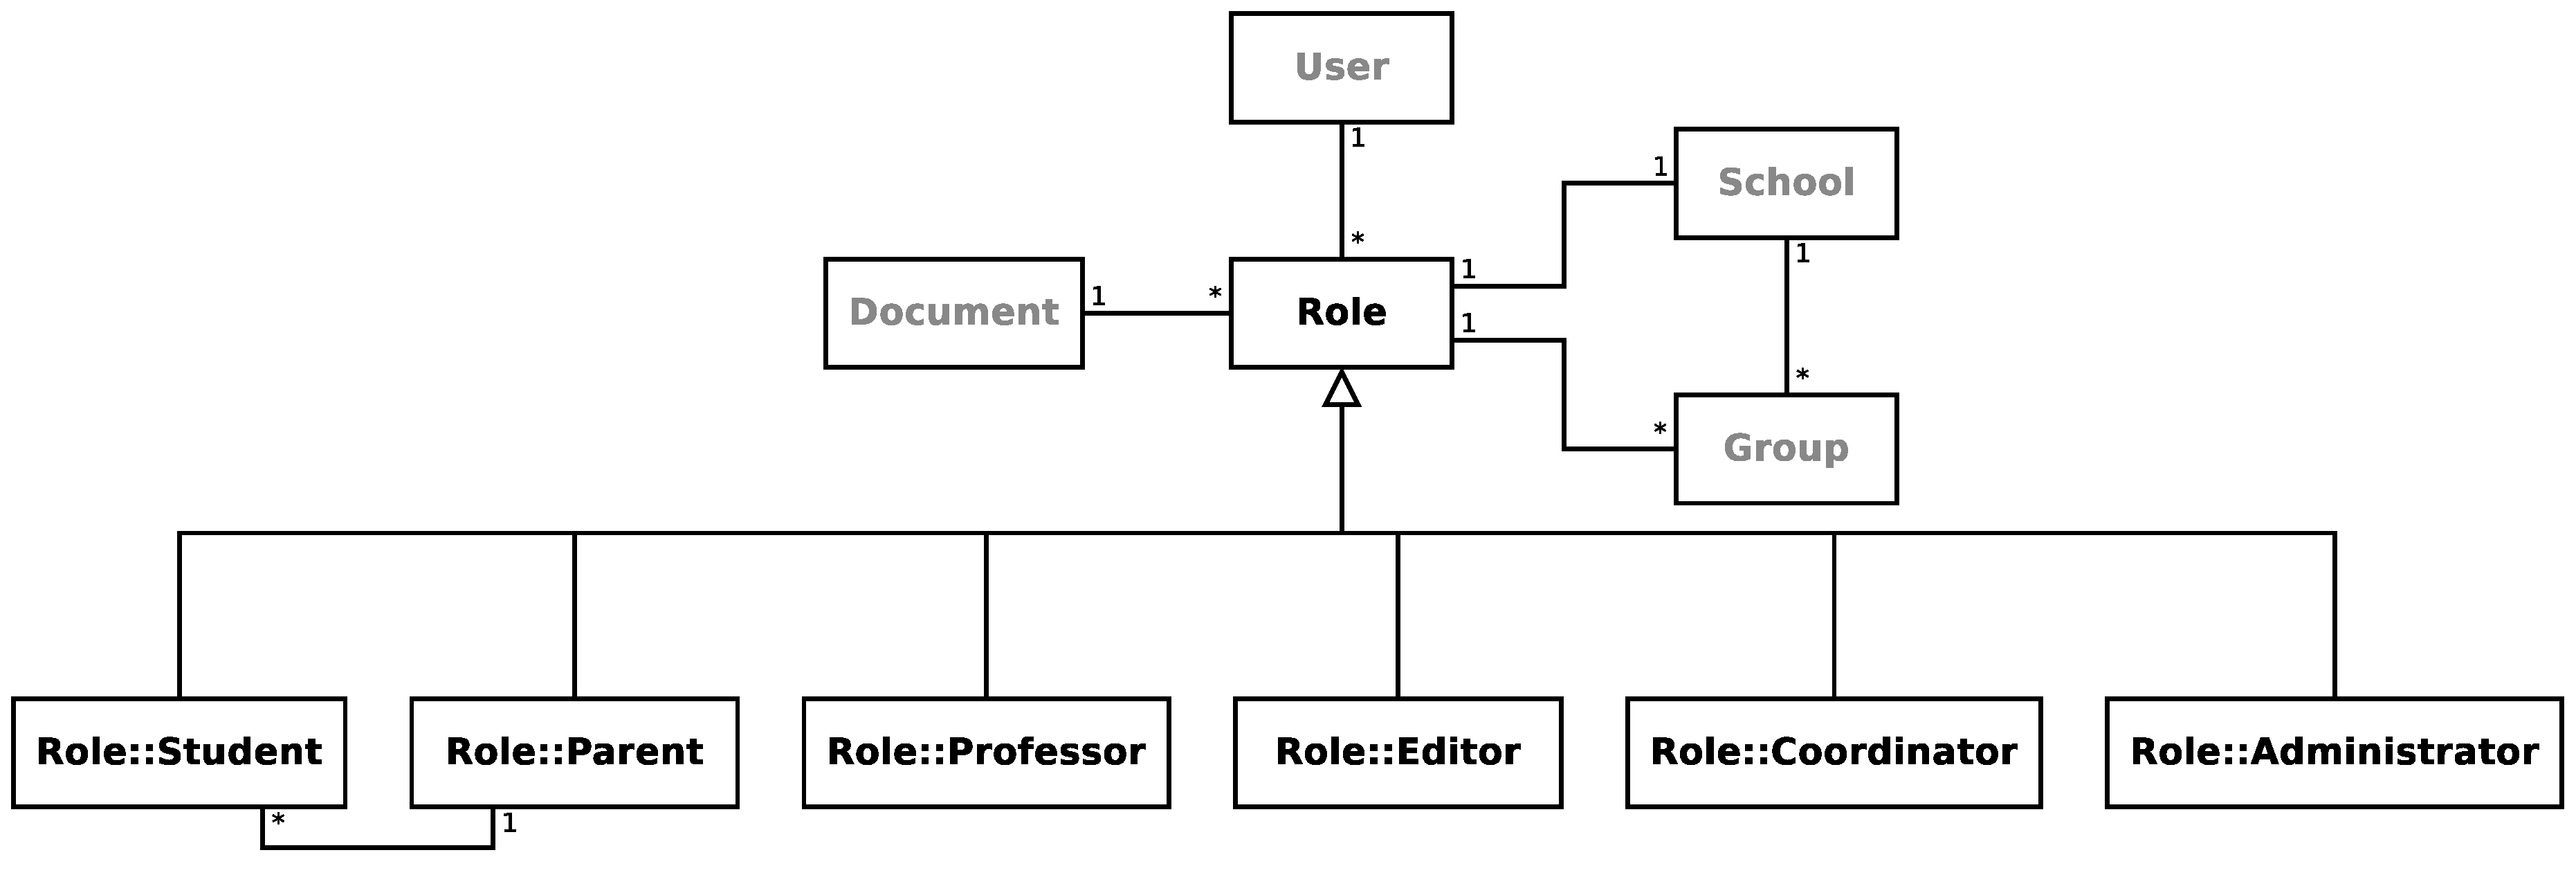
\includegraphics[width=160mm]{user_roles_conceptual}
  \caption{Conceptual User Roles Model}
  \label{fig:user_roles_conceptual}
\end{figure}

\subsection{Implementation}\label{sec:fa_roles_implementation}

\subsection{Impact Analysis}\label{sec:fa_roles_impact_analysis}
